%!TEX root = ../rapport.tex
%!TEX encoding = UTF-8 Unicode
\chapter{Outil de contrôle et de dimensionnement}
Cette section présente l'interface de contrôle et de dimensionnement des simulateurs PSim et SPS.

En premier lieu, l'outil de contrôle doit connaître les différentes simulations disponibles ainsi que les chemins d'accès pour y accéder. La figure \ref{outil1} présente les différentes informations nécessaires pour le bon fonctionnement de l'outil.

 \begin{figure}[htb]
 \centering
 \makebox[\textwidth][c]{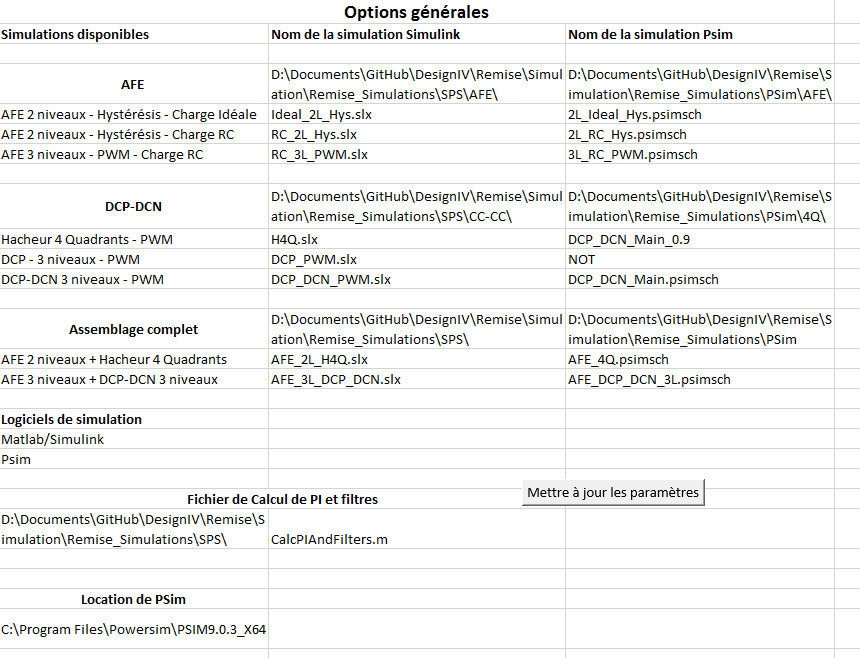
\includegraphics[width=0.95\textwidth]{fig/outil1.png}}
 \caption{Préprogrommation de l'outil de contrôle et de dimensionnement}
 \label{outil1}
 \end{figure}

Par la suite, une fois les informations des simulations mises en place, il suffit de choisir la simulation qui doit être lancée, de choisir le simulateur cible et d'entrer les différents paramètres de simulation. La figure \ref{outil2} présente l'interface de lancement et de programmation des paramètres.

 \begin{figure}[htb]
 \centering
 \makebox[\textwidth][c]{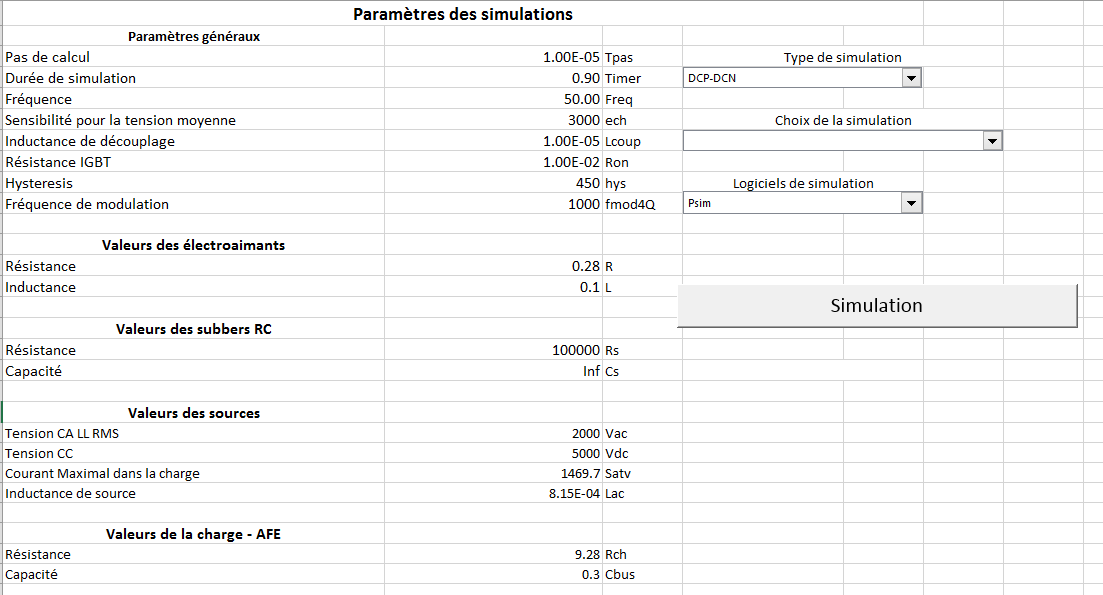
\includegraphics[width=0.95\textwidth]{fig/outil2.png}}
 \caption{Interface de lancement et de programmation des paramètres}
 \label{outil2}
 \end{figure}

 Cet outil permet de gagner un temps précieux lors de l'enchaînement rapide des simulations, car tous les paramètres capitaux sont regroupés au même endroit. De plus, comme l'outil permet de contrôler les deux plateformes de simulateurs, les valeurs vont être les mêmes d'une plateforme vers l'autre.
